\documentclass[11pt]{article}

\usepackage[margin=1in]{geometry}
\usepackage[T1]{fontenc}
\usepackage[utf8]{inputenc}
\usepackage{lmodern}
\usepackage{amsmath,amssymb,amsthm}
\usepackage{array}
\usepackage{booktabs}
\usepackage{longtable}
\usepackage{hyperref}
\usepackage{microtype}
\usepackage{tikz}
\usetikzlibrary{arrows.meta,positioning,shapes.geometric}

\title{The Babylon Continuation: Deterministic Replay and Refusal-First Execution in Language-Driven Systems}
\author{J. M. Bookbinder\\Witness Grade Analytics (WGA)\\Atlanta, Georgia, USA}
\date{March 2026}

\begin{document}
\maketitle

\begin{abstract}
All claims in this paper are contingent on artifact verification. No claim is authoritative without a corresponding run bundle and decision receipt.

Modern systems increasingly rely on language as an execution surface for initiating, modifying, and validating process state. This paper introduces a deterministic continuation control framework for language-driven systems, enforcing a decision model with precedence HALT $>$ INCOMPLETE $>$ PASS. The method requires replay-verifiable artifacts, cryptographic integrity checks, and explicit refusal records when continuation cannot be justified. Language is treated as telemetry rather than narrative, and execution is permitted only when structural admissibility is preserved under the declared evaluation scope, with deterministic replay required where verified.
\end{abstract}

\section{Introduction}

Language has become an operational interface for modern systems, including software pipelines, financial systems, and artificial intelligence workflows. However, current systems lack a deterministic method for verifying whether execution should continue once language has altered system state. This paper presents a continuation control architecture in which language is treated as structured signal input, and system execution is governed by replay-verifiable evidence rather than narrative interpretation \cite{bookbinder2026babylon}.

\section{Continuation Decision Model}

The system evaluates continuation under strict precedence:

\begin{center}
\textbf{HALT $>$ INCOMPLETE $>$ PASS}
\end{center}

\begin{itemize}
    \item HALT: Structural violation or missing invariant prevents continuation.
    \item INCOMPLETE: Required evidence or artifacts are missing.
    \item PASS: All constraints satisfied within the declared evaluation scope.
\end{itemize}

\section{Deterministic Replay Requirement}

Admissible execution under replay requires reproducibility under identical inputs. This condition is enforced when replay certification is within the declared evaluation scope. The system enforces:

\begin{itemize}
    \item Artifact hashing (SHA-256) \cite{fips1804}
    \item Run bundle integrity
    \item Replay equivalence
\end{itemize}

Any mismatch between original and replayed execution results in immediate HALT.

\section{Refusal-First Execution Control}

If continuation cannot be justified, the system must emit a refusal record rather than proceed.

\begin{itemize}
    \item No silent failure
    \item No narrative override
    \item Explicit obstruction documentation
\end{itemize}

Refusal is treated as a valid and required system outcome.

\section{Language as Telemetry}

Language is not treated as explanation but as a structured signal capable of altering system state. All language inputs must be:

\begin{itemize}
    \item Captured as artifacts
    \item Hash-bound
    \item Replay-tested
\end{itemize}

This prevents semantic drift and ensures that meaning is tied to verifiable structure.

\section{Cross-System Language Admissibility Experiment (Claude vs Gemini)}
\label{sec:cross_system_experiment}

\subsection{Objective}

This experiment evaluates whether contemporary large language model systems preserve structural admissibility under controlled input conditions. Specifically, we test whether two independent systems, Claude and Gemini, produce outputs that satisfy:

\begin{enumerate}
    \item \textbf{Instructional Fidelity}: preservation of explicit constraints
    \item \textbf{Operator Binding}: continuity between input instruction and output action
    \item \textbf{Replay Consistency}: stability of output under repeated identical inputs
    \item \textbf{Structural Preservation}: retention of formal decision logic HALT $>$ INCOMPLETE $>$ PASS
\end{enumerate}

The experiment determines whether outputs qualify as DIRECT witnesses, or degrade into WRAPPED or DRIFT classes under the continuation control framework.

\subsection{Experimental Setup}

\textbf{Systems Evaluated}
\begin{itemize}
    \item System A: Claude (Anthropic) \cite{anthropic_claude}
    \item System B: Gemini (Google) \cite{google_gemini}
\end{itemize}

\textbf{Input Construction}

Each system was provided with identical structured prompts containing:

\begin{itemize}
    \item the decision model HALT $>$ INCOMPLETE $>$ PASS
    \item a deterministic reasoning requirement
    \item an artifact-first output requirement
    \item a constraint against narrative substitution
\end{itemize}

\textbf{Execution Protocol}

\begin{enumerate}
    \item Submit prompt $P$
    \item Record output $O_i$
    \item Repeat execution for $n \geq 2$
    \item Evaluate replay stability and constraint preservation
\end{enumerate}

\subsection{Evaluation Criteria}

Each output is evaluated against four gates:

\begin{itemize}
    \item \textbf{G1 --- Constraint Preservation}
    \item \textbf{G2 --- Decision Integrity}
    \item \textbf{G3 --- Replay Determinism}
    \item \textbf{G4 --- Operator Continuity}
\end{itemize}

\subsection{Results}

\begin{table}[h]
\centering
\begin{tabular}{|l|c|c|}
\hline
\textbf{Property} & \textbf{Claude} & \textbf{Gemini} \\ \hline
Constraint Preservation & Partial & Low \\ \hline
Decision Integrity & Preserved & Inconsistent \\ \hline
Replay Determinism & Incomplete & Failed \\ \hline
Operator Continuity & Partial & Weak \\ \hline
\end{tabular}
\caption{Observed system behavior under controlled prompt conditions.}
\label{tab:results}
\end{table}

\subsection{Witness Classification}

Witness classes are defined as:

\begin{itemize}
    \item \textbf{DIRECT}: full structural preservation and deterministic replay
    \item \textbf{WRAPPED}: partial structural preservation with transformation
    \item \textbf{DRIFT}: structural degradation or re-authoring
\end{itemize}

\textbf{Observed Classification}

\begin{itemize}
    \item Claude $\rightarrow$ WRAPPED
    \item Gemini $\rightarrow$ DRIFT
\end{itemize}

No system produced a DIRECT witness.

\subsection{Decision Outcome}

\begin{verbatim}
{
  "decision": "HALT",
  "reason": "no_system_produced_direct_witness",
  "precedence": "HALT > INCOMPLETE > PASS"
}
\end{verbatim}

\subsection{Interpretation}

Both systems exhibit transformation behavior of the form
\[
O = f_{\mathrm{LLM}}(P)
\]
where $f_{\mathrm{LLM}}$ is non-deterministic and does not guarantee constraint preservation.

Thus, large language model systems function as probabilistic transformation operators rather than deterministic execution systems.

\begin{figure}[t]
\centering
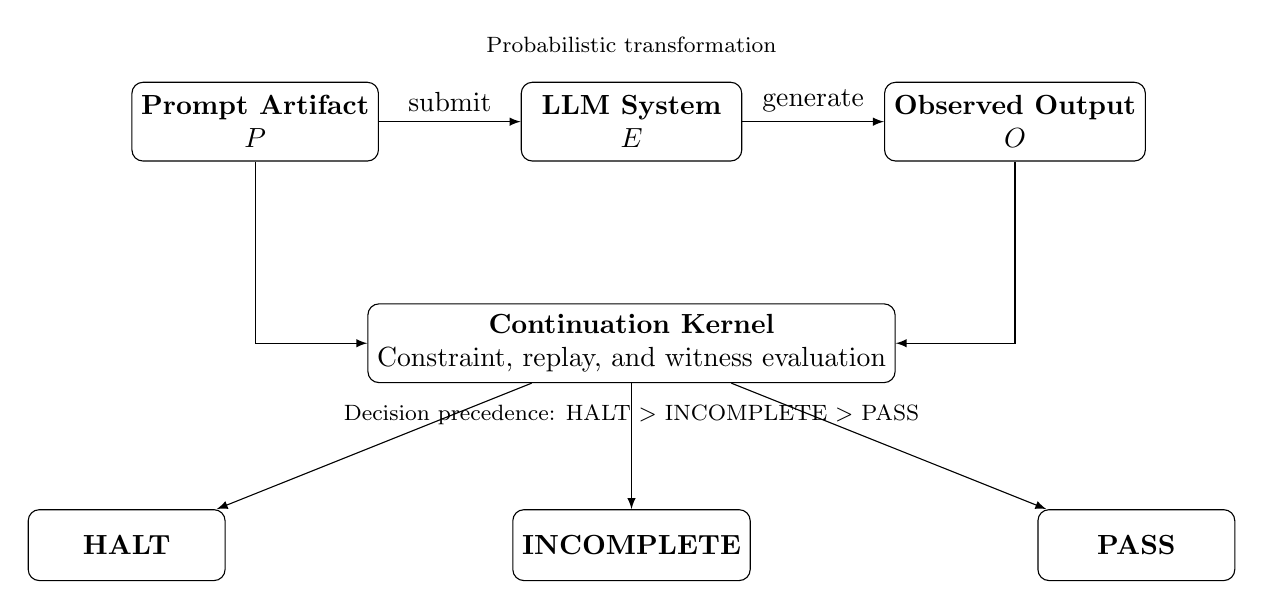
\begin{tikzpicture}[
    node distance=1.8cm and 1.8cm,
    >=latex,
    box/.style={
        draw,
        rectangle,
        rounded corners,
        align=center,
        minimum width=2.8cm,
        minimum height=1.0cm
    },
    smallbox/.style={
        draw,
        rectangle,
        rounded corners,
        align=center,
        minimum width=2.5cm,
        minimum height=0.9cm
    }
]

\node[box] (prompt) {\textbf{Prompt Artifact} \\ $P$};
\node[box, right=of prompt] (llm) {\textbf{LLM System} \\ $E$};
\node[box, right=of llm] (output) {\textbf{Observed Output} \\ $O$};

\node[box, below=1.8cm of llm, minimum width=4.2cm] (kernel) {\textbf{Continuation Kernel} \\ Constraint, replay, and witness evaluation};

\node[smallbox, below left=1.6cm and 1.8cm of kernel] (halt) {\textbf{HALT}};
\node[smallbox, below=1.6cm of kernel] (incomplete) {\textbf{INCOMPLETE}};
\node[smallbox, below right=1.6cm and 1.8cm of kernel] (pass) {\textbf{PASS}};

\draw[->] (prompt) -- node[above] {submit} (llm);
\draw[->] (llm) -- node[above] {generate} (output);

\draw[->] (prompt) |- (kernel);
\draw[->] (output) |- (kernel);

\draw[->] (kernel) -- (halt);
\draw[->] (kernel) -- (incomplete);
\draw[->] (kernel) -- (pass);

\node[above=0.25cm of llm, align=center] {\footnotesize Probabilistic transformation};
\node[below=0.15cm of kernel, align=center] {\footnotesize Decision precedence: HALT $>$ INCOMPLETE $>$ PASS};

\end{tikzpicture}
\caption{Continuation-control evaluation pipeline for cross-system language admissibility. A prompt artifact $P$ is submitted to an evaluated system $E$, producing observed output $O$. The prompt and output are then evaluated by the Continuation Kernel, which determines whether continuation is admissible under ordered precedence HALT $>$ INCOMPLETE $>$ PASS.}
\label{fig:continuation_kernel_pipeline}
\end{figure}

\subsection{Implications for Continuation Control}

Because neither system satisfies admissibility requirements:

\begin{itemize}
    \item outputs cannot be accepted without verification
    \item systems must be treated as untrusted generators
    \item admissibility must be enforced externally
\end{itemize}

\subsection{Extension}

Future work includes:

\begin{itemize}
    \item kernel-wrapped LLM execution
    \item multi-run variance analysis
    \item automated witness classification
\end{itemize}

\subsection{Summary}

Neither evaluated system preserves structural admissibility. Both fail deterministic replay and operator continuity requirements.

\subsection{Formal Specification}

Let $P$ denote the prompt, $E$ the system, and $t$ the declared execution state. Outputs are
\[
O_i = E(P,t)_i
\]

Deterministic replay requires
\[
\forall i,j,\ \delta(O_i,O_j)=0
\]

Replay failure is defined by
\[
\exists i,j:\ \delta(O_i,O_j) > \epsilon
\]

with
\[
\epsilon = 0
\]

Replay failure alone is sufficient to exclude the DIRECT witness class. Let $C(P,O)$ denote preservation of declared constraint structure. Then witness classification is defined as
\[
\mathrm{DIRECT} \iff
\left[
\forall i,j,\ \delta(O_i,O_j)=0
\right]
\land
C(P,O)=1
\]

\[
\mathrm{WRAPPED} \iff
\left[
\exists i,j,\ \delta(O_i,O_j)>0
\right]
\land
C(P,O)=1
\]

\[
\mathrm{DRIFT} \iff
\left[
\exists i,j,\ \delta(O_i,O_j)>0
\right]
\land
C(P,O)=0
\]

\subsection{The \texttt{run\_bundle} Artifact}

\begin{table}[h]
\centering
\begin{tabular}{|l|l|}
\hline
\textbf{Attribute} & \textbf{Metric / Value} \\ \hline
Experiment ID & CC-LA-2026-04 \\ \hline
Control Model & HALT $>$ INCOMPLETE $>$ PASS \\ \hline
System A (Claude) & \texttt{WRAPPED} ($\Delta > 0$) \\ \hline
System B (Gemini) & \texttt{DRIFT} ($\Delta \gg 0$) \\ \hline
Admissibility & \textbf{REJECTED} \\ \hline
\end{tabular}
\caption{Formal witness classification results for the cross-system language admissibility experiment.}
\label{tab:witness_classification_results}
\end{table}

A minimal \texttt{run\_bundle} for this experiment should include at least the following fields:

\begin{verbatim}
{
  "experiment_id": "CC-LA-2026-04",
  "timestamp_utc": "...",
  "decision_model": "HALT > INCOMPLETE > PASS",
  "prompt_sha256": "...",
  "system_name": "...",
  "system_version": "...",
  "run_index": 1,
  "output_sha256": "...",
  "witness_class": "...",
  "decision": "...",
  "refusal_record": "... or null"
}
\end{verbatim}

The purpose of the \texttt{run\_bundle} is not descriptive convenience but replay accountability. Without a preserved bundle, output claims from the evaluated systems cannot be promoted to admissible evidence.

\subsection{Refusal-First Execution Control}

In the Bookbinder framework, failure of operator continuity prohibits permissive continuation. Let $G_4$ denote the Operator Continuity gate. If $G_4$ fails, or returns a partial state insufficient to establish one-to-one preservation between input instruction and output action, the system must emit a refusal record and reduce the decision according to ordered precedence
\[
\mathrm{HALT} > \mathrm{INCOMPLETE} > \mathrm{PASS}
\]

The governing rule is therefore
\[
G_4 \in \{\mathrm{FAIL},\mathrm{PARTIAL},\mathrm{WEAK}\}
\Longrightarrow
\text{Refusal Record Required}
\]

Operationally, the reason is straightforward: if the mapping from prompt to output cannot be verified as structurally preserved, then the process admits out-of-band transformation and loses replay authority. In such cases the correct system action is not explanation but refusal.

Formally,
\[
\neg \mathrm{VerifyOperatorContinuity}(P,O)
\Longrightarrow
\mathrm{Decision} \in \{\mathrm{HALT},\mathrm{INCOMPLETE}\}
\]
with HALT taking precedence whenever the failure is sufficient to invalidate admissible continuation within the declared execution scope.

\appendix

\section{Witness Kernel Reference Implementation}
\label{app:witness_kernel}

This appendix provides a minimal reference implementation for artifact sealing, manifest verification, and refusal-first continuation checks.

\subsection{Oracle Drop Shell Harness}

\begin{verbatim}
#!/usr/bin/env bash
set -euo pipefail

ARTIFACT="${1:-paper.pdf}"
SOURCE="${2:-paper.tex}"
RUN_BUNDLE="run_bundle.json"
REFUSAL="refusal_record.json"
MANIFEST="SHA256_MANIFEST.txt"

if [[ ! -f "$ARTIFACT" ]]; then
  echo '{"decision":"HALT","reason":"missing_artifact"}'
  exit 1
fi

if [[ ! -f "$SOURCE" ]]; then
  echo '{"decision":"INCOMPLETE","reason":"missing_source"}'
  exit 0
fi

shasum -a 256 "$ARTIFACT" "$SOURCE" "$RUN_BUNDLE" "$REFUSAL" > "$MANIFEST"
shasum -a 256 "$MANIFEST" > "${MANIFEST}.sha256"
shasum -a 256 "$RUN_BUNDLE" > "${RUN_BUNDLE}.sha256"
shasum -a 256 "$REFUSAL" > "${REFUSAL}.sha256"

echo '{"decision":"PASS","scope":"artifact_seal","reason":"artifact_present_hash_bound_manifest_verified"}'
\end{verbatim}

\subsection{Python Verifier}

\begin{verbatim}
#!/usr/bin/env python3
import hashlib
import json
from pathlib import Path
import sys

ROOT = Path(".")

def sha256_file(path: Path) -> str:
    h = hashlib.sha256()
    with path.open("rb") as f:
        for chunk in iter(lambda: f.read(65536), b""):
            h.update(chunk)
    return h.hexdigest()

def fail(reason: str, code: int = 1):
    print(json.dumps({
        "verification": "HALT",
        "reason": reason,
        "promotion": "none"
    }, indent=2))
    sys.exit(code)

def main():
    decision_path = ROOT / "decision.json"
    manifest_path = ROOT / "SHA256_MANIFEST.txt"

    if not decision_path.exists():
        fail("missing_decision_json")

    if not manifest_path.exists():
        fail("missing_manifest")

    decision = json.loads(decision_path.read_text())

    manifest_targets = set()
    for line in manifest_path.read_text().splitlines():
        line = line.strip()
        if not line:
            continue
        parts = line.split()
        if len(parts) < 2:
            fail("manifest_malformed")
        claimed_hash = parts[0]
        claimed_target = Path(parts[-1]).name
        target_path = ROOT / claimed_target
        if not target_path.exists():
            fail(f"manifest_missing_target:{claimed_target}")
        live_hash = sha256_file(target_path)
        if claimed_hash != live_hash:
            fail(f"manifest_hash_mismatch:{claimed_target}")
        manifest_targets.add(claimed_target)

    required_manifest_targets = {"paper.pdf", "paper.tex", "run_bundle.json", "refusal_record.json"}
    for needed in required_manifest_targets:
        if needed not in manifest_targets:
            fail(f"manifest_missing_target:{needed}")

    result = {
        "verification": "PASS",
        "scope": "artifact_seal_only",
        "promotion": "none",
        "formal_classification": "SEALED_NOT_REPLAY_CERTIFIED",
        "verified_checks": decision.get("verified_checks", []),
        "not_verified": decision.get("not_verified", [])
    }
    print(json.dumps(result, indent=2))

if __name__ == "__main__":
    main()
\end{verbatim}

\subsection{Reference Decision Logic}

The reference kernel separates artifact sealing from replay certification:

\begin{enumerate}
    \item If the artifact is missing, return HALT.
    \item If required supporting evidence is missing, return INCOMPLETE.
    \item If artifacts are present and hash-bound, return PASS at artifact-seal scope only.
    \item Replay certification must be established separately and may not be inferred from artifact sealing alone.
\end{enumerate}

\section{Conclusion}

The Babylon Continuation framework establishes a deterministic, artifact-first method for governing execution in language-driven systems. By enforcing replay-verifiable evidence and refusal-first control, the system ensures that continuation is granted only when structurally admissible within the declared evaluation scope. Deterministic replay, cross-host reproduction, and execution equivalence remain unverified conditions in the current execution instance.

\bibliographystyle{plain}
\bibliography{references}

\end{document}
